\documentclass[border=3mm,tikz,preview]{standalone}
\usetikzlibrary{intersections}
\usepackage{amsmath}
\usetikzlibrary{shapes.misc}

\tikzset{cross/.style={cross out, draw=black, minimum size=2*(#1-\pgflinewidth), inner sep=0pt, outer sep=0pt},
	%default radius will be 1pt. 
	cross/.default={2pt}}

\begin{document}
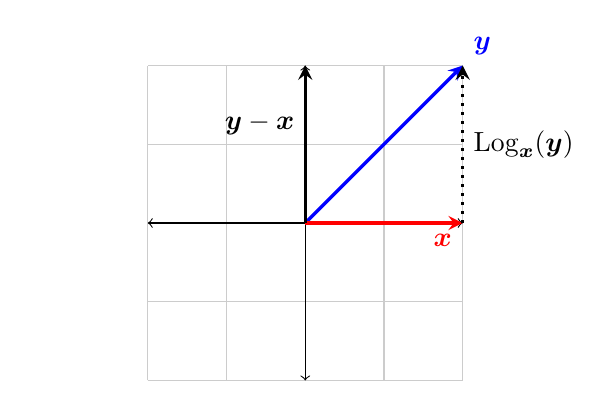
\begin{tikzpicture}
		\draw[line width=1.25pt,-stealth, dotted, white] (-2, 0) -- (-2, 2) node[anchor=east, yshift = -1cm]{$\mathrm{Log}_{\boldsymbol{x}}(\boldsymbol{y})$};
	\draw[thin,gray!40] (-2,-2) grid (2,2);
	\draw[<->] (-2,0)--(2,0);
	\draw[<->] (0,-2)--(0,2);
	\draw[line width=1.25pt,blue,-stealth](0,0)--(2,2) node[anchor=south west]{$\boldsymbol{y}$};
	\draw[line width=1.25pt,red,-stealth](0,0)--(2, 0) node[anchor=north east]{$\boldsymbol{x}$};
	\draw[line width=1.25pt,-stealth, dotted] (2, 0) -- (2, 2) node[anchor=west, yshift = -1cm]{$\mathrm{Log}_{\boldsymbol{x}}(\boldsymbol{y})$};
	\draw[line width=1.25pt,-stealth] (0, 0) -- (0, 2) node[anchor=east, yshift=-0.75cm]{$\boldsymbol{y} - \boldsymbol{x}$};
\end{tikzpicture}
\end{document}